\chapter{Waarskynlikheid}\fancyfoot[LO,RE]{Fokus Area: Wiskunde}
% 
% \section{Inleiding}
Ons gebruik waarskynlikheid om gebeuertenisse met onsekerheid te beskrywe. Wanner mens 'n sny brood laat val, dan weet jy nie of dit met die botterkant bo of onder gaan land nie. Wanneer jou voorkeur-sportspan speel weet jy nie of hulle gaan wen of verloor nie. Wanneer die weerman aandui dat daar 'n $40\%$ kans is vir re\"en more is, dan mag jy nat word of nie.  Onsekerheid kom tot 'n mate voor in byna elke gebeurtenis om ons en in elke besluit wat ons maak.\par

Ons sal in hierdie hoofstuk sien dat al hierdie onsekerhede beskryf kan word deur gebruik van die reels van waarskynlikheid en dat ons definitiewe besluite kan neem oor onsekere prosesse.
\par


Ons gaan drie voorbeelde gebruik om jou te help om die verskillende terme in waarskynlikheidsteorie te verstaan: 'n muntstuk opskiet, dobbelstene rol en 'n sokkerwedstryd.\par
\chapterstartvideo{VMbxk}

\Definition{Eksperiment}{'n Eksperiment verwys na 'n proses met onsekerheid}

\Definition{Uitslag}{Die uitslag van 'n eksperiment is 'n enkele resultaat van daardie eksperiment.}

\paragraph{Eksperiment 1} 'n Muntstuk word opgeskiet en dit land met of kruis (K) of munt (M) bo. 'n Voorbeeld van die uitslag van 'n muntstuk opskiet: dit land met munt bo:

\def\coinheads{\draw (0,0) circle (1cm); \draw (0,0) circle (0.8cm); \draw (0,0) node {\Huge\textbf{H}};}
\def\cointails{\draw (0,0) circle (1cm); \draw (0,0) circle (0.8cm); \draw (0,0) node {\Huge\textbf{T}};}

\begin{figure}[h]
  \begin{center}
    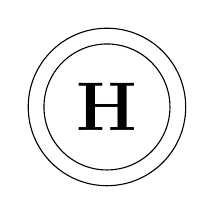
\begin{tikzpicture}
      \coinheads
    \end{tikzpicture}
  \end{center}
%   \caption{}
\end{figure}

\paragraph{Eksperiment 2} Twee dobbelstene word gerol en die aantal kolletjies bymekaar getel. 'n Voorbeeld van die uitslag van twee dobbelstene wat gerol word:

\begin{figure}[h]
  \begin{center}
    \begin{tikzpicture}
      \makedie{3}{shift={(-1,0)},rotate=10}
      \makedie{5}{shift={(1,0)},rotate=-20}
    \end{tikzpicture}
  \end{center}
%   \caption{}
\end{figure}

\paragraph{Eksperiment 3} Twee sokkerspanne speel 'n wedstryd en ons stel belang in die eindtelling.'n Voorbeeld van die uitslag van 'n sokkerwedstryd:

\begin{figure}[h]
  \begin{center}
    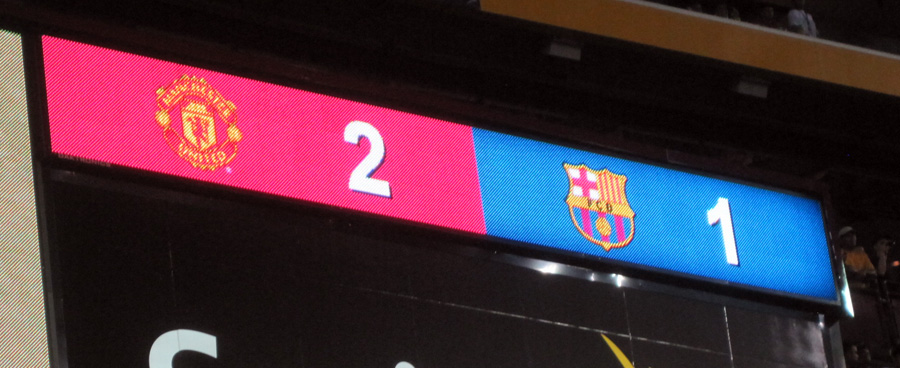
\includegraphics[width=3in]{Gr10-Probability-images/5996076302_412ec8d8d0_o.jpg}
 \\
  \begin{caption*}{(prentjie deur apasciuto on Flickr.com)}\end{caption*}
 \end{center}
\end{figure}

\Definition{Monsterrruimte}{Die monsterruimte van 'n versameling is die versameling van al die moontlike uitslae van daardie eksperiment. Die monsterruimte word aangedui deur die simbool \(S\) en die grootte van die monsterruimte (die som van al die moontlike uitkomste) word aangedui deur \(n(S)\).}

Selfs al stel ons gewoonlik net belang in die enkele uitkoms van 'n eksperiment, het ons ook nodig om te weet wat die ander uitkomste sou kon wees. Kom ons kyk na die monsterruimtes van ons drie eksperimente.

\paragraph{Eksperiment 1} Aangesien 'n muntstuk net op twee maniere kan land (ons ignoreer die waarskynlikheid dat die munstuk op sy kant kan land),  is die monsterruimte die versameling \(S=\{\mbox{H}; \mbox{T}\}\). Die grootte van die monsterruimte is \(n(S)=2\).

\begin{figure}[H]
  \begin{center}
  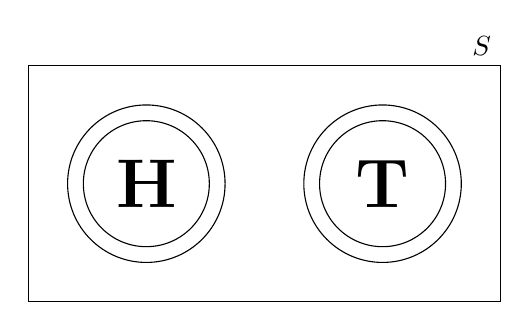
\begin{tikzpicture}
    \begin{scope}[xshift=-1.5cm]
      \coinheads
    \end{scope}
    \begin{scope}[xshift=+1.5cm]
      \cointails
    \end{scope}
    \draw (-3, -1.5) rectangle (3, 1.5) node[anchor=south east] {$S$};
  \end{tikzpicture}
  \end{center}
%   \caption{Sample space of a coin toss.}
\end{figure}

\paragraph{Eksperiment 2} Elkeen van die dobbelstene kan land op 'n nommer van $1$ tot $6$. In hierdie eksperiment is die monsterruimte van al die moontlike uitkomste elke moontlike kombinasie van die $6$ nommers op die eerste dobbelsteen met die $6$ nommers op die tweede dobbelsteen. Dit gee 'n totaal van \(n(S) = 6 \times 6
= 36\) uitkomste. Die figuur hieronder wys al die uitkomste in die monsterruimte:

\begin{figure}[h]
\begin{center}
\begin{tikzpicture}
  \begin{scope}[scale=0.5]
  \foreach \x in {1, ..., 6} {
    \foreach \y in {1, ..., 6} {
      \pgfmathparse{15*rand} \let\rot\pgfmathresult
      \makediesmall{\x}{shift={(4cm*\x-0.66cm,-2cm*\y)},rotate=\rot}
      \pgfmathparse{15*rand} \let\rot\pgfmathresult
      \makediesmall{\y}{shift={(4cm*\x+0.66cm,-2cm*\y)},rotate=\rot}
    }
  }
  \draw[thick] (2.5cm-0.66cm, -0.5cm) rectangle (25.5cm+0.66cm, -13.5cm);
  \draw (25.5cm+0.66cm, -0.5cm) node[anchor=south east] {$S$};
  \end{scope}
\end{tikzpicture}
\end{center}
%   \caption{Monsterruimte van die rol van twee dobbelstene}
\end{figure}

\paragraph{Eksperiment 3} Elke sokkerspan kan 'n heelgetal telling kry vanaf $0$ opwaarts. Ons verwag gewoonlik nie 'n ho\"er telling as $5$ doele nie, maar daar is geen rede hoekom dit nie kan gebeur nie. Die monsterruimte van hierdie eksperiment bestaan dus uit al die moontlike kombinasies van twee nie-negatiewe heelgetalle. Die figuur hieronder wys al die moontlikhede. Ons begrens nie die tellings van enige span nie, dus is hierdie monsterrumte oneindig groot:

\begin{figure}[h]
\begin{center}
  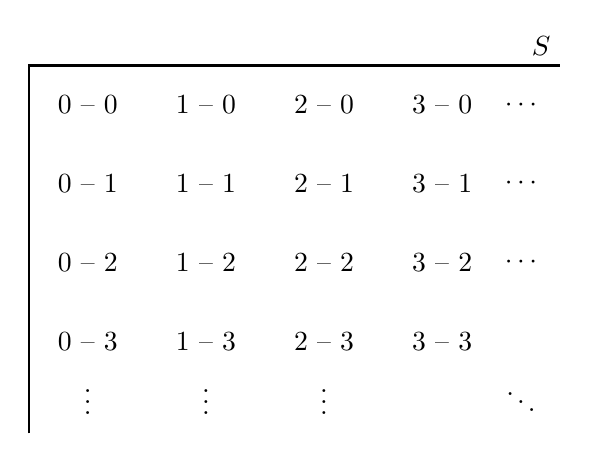
\begin{tikzpicture}
    \foreach \x in {0, ..., 3} {
      \foreach \y in {0, ..., 3} {
        \draw (\x*1.5cm,-\y) node {\x\ --\ \y};
      }
    }
    \foreach \x in {0, ..., 2} {
      \draw (\x*1.5cm,-3.67cm) node {$\vdots$};
    }
    \foreach \y in {0, ..., 2} {
      \draw (5.5cm,-\y) node {$\cdots$};
    }
    \draw (5.5cm,-3.67cm) node {$\ddots$};

    \draw[thick] (-0.75cm, -4.17cm) -- (-0.75, 0.5cm) -- (6cm, 0.5cm);
    \draw (6cm, 0.5cm) node[anchor=south east] {$S$};
  \end{tikzpicture}
\end{center}
%   \caption{Monsterruimte van die eindtelling van 'n sokkerwedstryd.}
\end{figure}

\Definition{Gebeurtenis}{'n Gebeurtenis is 'n spesifieke versameling van uitkomste van 'n eksperiment waarin jy belangstel. 'n Gebeurtenis word aangedui deur die letter \(E\) en die aantal uitkomste van die gebeurtenis met \(n(E)\).}

\paragraph{Eksperiment 1} Gestel ons wil h\^e die munstuk moet land met kruis bo. Hier het die gebeurtenis net een uitkoms, naamlik
\(E=\{\mbox{H}\}\), \(n(E)=1\).

\paragraph{Eksperiment 2} Gestel ons stel belang in die geval dat die som van die twee dobbelstene $8$ is. In hierdie geval is die versameling van die gebeuretenis
$E=\{($\raisebox{-2pt}{\begin{tikzpicture}
  \begin{scope}[scale=0.333]
    \makediegeneral{2}{xshift=-0.7cm}{0.175cm*0.333}
    \makediegeneral{6}{xshift=+0.7cm}{0.175cm*0.333}
  \end{scope}
\end{tikzpicture}}$);($\raisebox{-2pt}{\begin{tikzpicture}
  \begin{scope}[scale=0.333]
    \makediegeneral{3}{xshift=-0.7cm}{0.175cm*0.333}
    \makediegeneral{5}{xshift=+0.7cm}{0.175cm*0.333}
  \end{scope}
\end{tikzpicture}}$);($\raisebox{-2pt}{\begin{tikzpicture}
  \begin{scope}[scale=0.333]
    \makediegeneral{4}{xshift=-0.7cm}{0.175cm*0.333}
    \makediegeneral{4}{xshift=+0.7cm}{0.175cm*0.333}
  \end{scope}
\end{tikzpicture}}$);($\raisebox{-2pt}{\begin{tikzpicture}
  \begin{scope}[scale=0.333]
    \makediegeneral{5}{xshift=-0.7cm}{0.175cm*0.333}
    \makediegeneral{3}{xshift=+0.7cm}{0.175cm*0.333}
  \end{scope}
\end{tikzpicture}}$);($\raisebox{-2pt}{\begin{tikzpicture}
  \begin{scope}[scale=0.333]
    \makediegeneral{6}{xshift=-0.7cm}{0.175cm*0.333}
    \makediegeneral{2}{xshift=+0.7cm}{0.175cm*0.333}
  \end{scope}
\end{tikzpicture}}$)\}$
want dit bevat al die moontlike maniere om $8$ kolletjies te kry met $2$ dobbelstene.
Die grootte van die gebeuretenis se versameling is \(n(E)=5\).

%Ons kan hierdie ook grafies voorstel deur 'n lyn te trek om die uitkomste waarin ons belangstel.
%FIGURE: Monsterruimte met 'n geslote kromme om die versameling van die gebeurtenis.

\paragraph{Eksperiment 3} Ons stel belang om te weet of die eerste span gaan wen. Daarvoor moet die eerste telling hoer wees as die tweede telling.
\[E=\{(1;0);(2;0);(2;1);(3;0);(3;1);(3;2);\ldots\}\]
Hierdie gebeurtenis-versameling is oneindg groot.

%FIGURE: Monsterruimte met 'n oop kromme om die gebeutenis-versameling. 

\section{Teoretiese waarskynlikheid}
\Definition{Waarskynlikheid}{'n Waarskynlikheid is 'n re\"ele getal tussen $0$ en $1$ wat beskryf hoe waarskynlik dit is dat die gebeurtenis sal plaasvind.}
\begin{itemize}
\item 'n Waarskynlikheid van $0$ beteken dat die gebeurtenis nooit sal plaasvind nie.
\item 'n Waarskynlikheid van $1$ beteken dat die gebeurtenis altyd sal plaasvind.
\item 'n Waarskynlikheid van $0,5$ beteken dat die gebeurtenis die helfte van die tyd sal plaasvind, of $1$ keer uit elke $2$.
\end{itemize}



Wanneer al die moontlike uitkomste van 'n eksperiment ewekansig is kan ons die pesiese teoretiese waarskynlikheid van die gebeurtenis bereken. Die waarskynlikheid van 'n gebeurtenis is die verhouding tussen die aantal uitkomste van die eksperiment en die grootte van die monsterruimte.
\[P(E) = \frac{n(E)}{n(S)}\] \par

\mindsetvid{Calculating probabilities}{VMbzp}
\begin{wex}{Teoretiese waarskynlikhede}{
Wat is die teoretiese waarskynlikheid van elk van die gebeurtenisse in die eerste twee van ons drie eksperimente?
}{
  \westep{Skryf die grootte van die monsterruimte neer}

  
  Eksperiment 1: $n(S) = 2$\\
 Eksperiment 2: $n(S) = 36$\\
  
  
  \westep{Skryf die grootte van die gebeurtenis-versameling neer}


  Eksperiment 1: $n(E) = 1$\\
 Eksperiment 2: $n(E) = 5$\\


  \westep{Bereken die teoretiese waarskynlikheid}


  Eksperiment 1: $P(E) = \frac{n(E)}{n(S)} = \frac{1}{2} = 0,5$\\
  Eksperiment 2: $P(E) = \frac{n(E)}{n(S)} = \frac{5}{36} = 0,13\dot{8}$\\
}
\end{wex}

Let daarop dat ons nie die teoretiese waarskynlikheid van die derde eksperiment in ag neem nie. Die derde eksperiment verskil van die eerste twee op 'n belangrike wyse, naamlik dat al die moontlike uitkomste (eindtellings) nie ewekansig is nie. Ons weet, byvoorbeeld, dat 'n sokkertelling van $1$--$1$ vry algemeen voorkom, terwyl 'n telling van $11$--$15$ uiters selde voorkom. Omdat al die uitkomste nie ewekansig is nie, kan ons nie die verhouding tussen \(n(E)\) en \(n(S)\) gebruik om die teoretiese waarskynlikheid van 'n span om te wen te bereken nie.
%  (\textbf{Interessante feit:} Die rekord vir die meeste doele aangeteken deur beide spanne in die FIFA wereldbeker is $12$. Hierdie het gebeur in $1954$ in die wedstryd tussen Oostenryk en Switserland, waar die eindtelling $7$--$5$ was.)

\begin{exercises}{}
{
  \begin{enumerate}[itemsep=5pt, label=\textbf{\arabic*}.]
  \item 'n Sak bevat $6$ rooi, $3$ blou, $2$ groen en $1$ wit
    balle. 'n Ball word lukraak gekies. Wat is die waarskynlikheid van die volgende:
    \begin{enumerate}
    \item rooi
    \item blou of wit
    \item nie groen
    \item nie groen of rooi
    \end{enumerate}
  \item 'n Speelkaart word lukraak gekies uit 'n pak van $52$ kaarte. Wat is die waarskynlikheid van die volgende:
    \begin{enumerate}

    \item die $2$ van harte
    \item 'n rooi kaart
    \item 'n prentkaart
    \item 'n 'Ace' getal
    \item 'n nommer kleiner as $4$
    \end{enumerate}

  \item Ewe getalle in die interval $2$ tot $100$ word op kaarte geskryf. Wat is
    die waarskynlikheid om 'n veelvoud van $5$ op 'n lukraak wyse te kies?
  \end{enumerate}

\insertpracticeinfo{3}
}
\end{exercises}

\section{Relatiewe frekwensie}

\Definition{Relatiewe frekwensie}{Die relatiewe frekwensie van 'n gebeurtenis word gedefinieer as die aantal kere wat die gebeurtenis voorkom in 'n aantal eksperimente, gedeel deur die aantal eksperimente.}

Die relatiewe frekwensie is 'n eksperimentele syfer, nie 'n teoretiese syfer nie. 'n Eksperiment moet 'n aantal kere herhaal word en die voorkoms van die gebeurtenis in die gebeurtenis-veresameling getel word. Omdat dit eksperimenteel is, is dit moontlik om telkens verskillende relatiewe frekwensies te kry met herhaling van die eksperiment.\par

\mindsetvid{Relative frequency}{VMbzy}

\begin{wex}{Relatiewe frekwensie en teoretiese waarskynlikheid}{
  Ons skiet 'n muntstuk $30$ keer op en beskou die uitkomste. Die resultate is in die tabelle hieronder.
%english in table below
  \begin{center}
    \begin{tabular}{lc@{\hspace{0.25cm}}c@{\hspace{0.25cm}}c@{\hspace{0.25cm}}c@{\hspace{0.25cm}}c@{\hspace{0.25cm}}c@{\hspace{0.25cm}}c@{\hspace{0.25cm}}c@{\hspace{0.25cm}}c@{\hspace{0.25cm}}c}
      \toprule
      toets   &  $1$ &  $2$ &  $3$ &  $4$ &  $5$ &  $6$ &  $7$ &  $8$ &  $9$ & $10$ \\
      uitkoms &  M &  K &  K &  K &  M &  K &  M &  M &  M &  K \\
      \midrule
      toets    & $11$ & $12$ & $13$ & $14$ & $15$ & $16$ & $17$ & $18$ & $19$ & $20$ \\
      uitkoms &  M &  K &  K &  M &  K &  K &  K &  M &  K &  K \\
      \midrule
      toets    & $21$ & $22$ & $23$ & $24$ & $25$ & $26$ & $27$ & $28$ & $29$ & $30$ \\
      uitkoms &  M &  M &  M &  K &  M &  K &  M &  K &  K &  K \\
      \bottomrule
    \end{tabular}
  \end{center}
  \vspace{8pt}\\

  Wat is die relatiewe frekwensie om munt te kry na elke toets en hoe vergelyk dit met die teoretiese waarskynlikheid om munt te kry?
}{
  \westep{Tel die aantal moontlike uitkomste}

  'n Positiewe uikoms is wanneer die uitkoms in ons versameling van gebeurtenisse is. Die tabel hieronder toon 'n lopende telling (na elke opskiet $t$) van die aantal positiewe uitkomste $p$ wat ons verkry het. Byvoorbeeld, na $t=20$ kere het ons $8$ keer munt en $12$ keer kruis, dus is die positiewe uitkoms-telling $p=8$.

  \begin{center}
    \begin{tabular}{cc@{\hspace{0.25cm}}c@{\hspace{0.25cm}}c@{\hspace{0.25cm}}c@{\hspace{0.25cm}}c@{\hspace{0.25cm}}c@{\hspace{0.25cm}}c@{\hspace{0.25cm}}c@{\hspace{0.25cm}}c@{\hspace{0.25cm}}c}
      \toprule
      $t$ &  $1$ &  $2$ &  $3$ &  $4$ &  $5$ &  $6$ &  $7$ &  $8$ &  $9$ & $10$ \\
      $p$ &  $1$ &  $1$ &  $1$ &  $1$ &  $2$ &  $2$ &  $3$ &  $4$ &  $5$ &  $5$ \\
      \midrule
      $t$ & $11$ & $12$ & $13$ & $14$ & $15$ & $16$ & $17$ & $18$ & $19$ & $20$ \\
      $p$ &  $6$ &  $6$ &  $6$ &  $7$ &  $7$ &  $7$ &  $7$ &  $8$ &  $8$ &  $8$ \\
      \midrule
      $t$ & $21$ & $22$ & $23$ & $24$ & $25$ & $26$ & $27$ & $28$ & $29$ & $30$ \\
      $p$ &  $9$ & $10$ & $11$ & $11$ & $12$ & $12$ & $13$ & $13$ & $13$ & $13$ \\
      \bottomrule
    \end{tabular}
  \end{center}
  \vspace{8pt}\\

  \westep{Bereken die relatiewe frekwensie}

  Die relatiewe frekwensie is gedefinieer as die verhouding tussen die aantal positiewe uitkomste en die totale aantal uitkomste,
  \[f=\frac{p}{t}\] 
%english
Die relatiewe frekwensie van om munt te kry, $f$, na $t$ muntstuk skiete is:


  \begin{center}
    \begin{tabular}{cc@{\hspace{0.25cm}}c@{\hspace{0.25cm}}c@{\hspace{0.25cm}}c@{\hspace{0.25cm}}c@{\hspace{0.25cm}}c@{\hspace{0.25cm}}c@{\hspace{0.25cm}}c@{\hspace{0.25cm}}c@{\hspace{0.25cm}}c}
      \toprule
      $t$ &  $1$ &  $2$ &  $3$ &  $4$ &  $5$ &  $6$ &  $7$ &  $8$ &  $9$ & $10$ \\
      $f$ & $1,00$ & $0,50$ & $0,33$ & $0,25$ & $0,40$ & $0,33$ & $0,43$ & $0,50$ & $0,56$ & $0,50$ \\
      \midrule
      $t$ & $11$ & $12$ & $13$ & $14$ & $15$ & $16$ & $17$ & $18$ & $19$ & $20$ \\
      $f$ & $0,55$ & $0,50$ & $0,46$ & $0,50$ & $0,47$ & $0,44$ & $0,41$ & $0,44$ & $0,42$ & $0,40$ \\
      \midrule
      $t$ & $21$ & $22$ & $23$ & $24$ & $25$ & $26$ & $27$ & $28$ & $29$ & $30$ \\
      $f$ & $0,43$ & $0,45$ & $0,48$ & $0,46$ & $0,48$ & $0,46$ & $0,48$ & $0,46$ & $0,45$ & $0,43$ \\
      \bottomrule
    \end{tabular}
  \end{center}
  \vspace{8pt}\\

Uit die laaste inskrywing in die tabel kan ons nou maklik die relatiewe frekwensie na 30 toetse aflees, naamlik $13/30 = 0,4\dot{3}$. Die relatiewe frekwensie is naby aan die waarskynlikheid van $0,5$. Oor die algemeen kom die relatiewe frekwensie nader aan die teoretiese frekwensie hoe meer toetse ons doen.\\
\\
'n Beter manier om die tabel van relatiewe frekwensie op te som is deur middel van 'n grafiek:

\begin{figure}[H]
  \begin{center}
    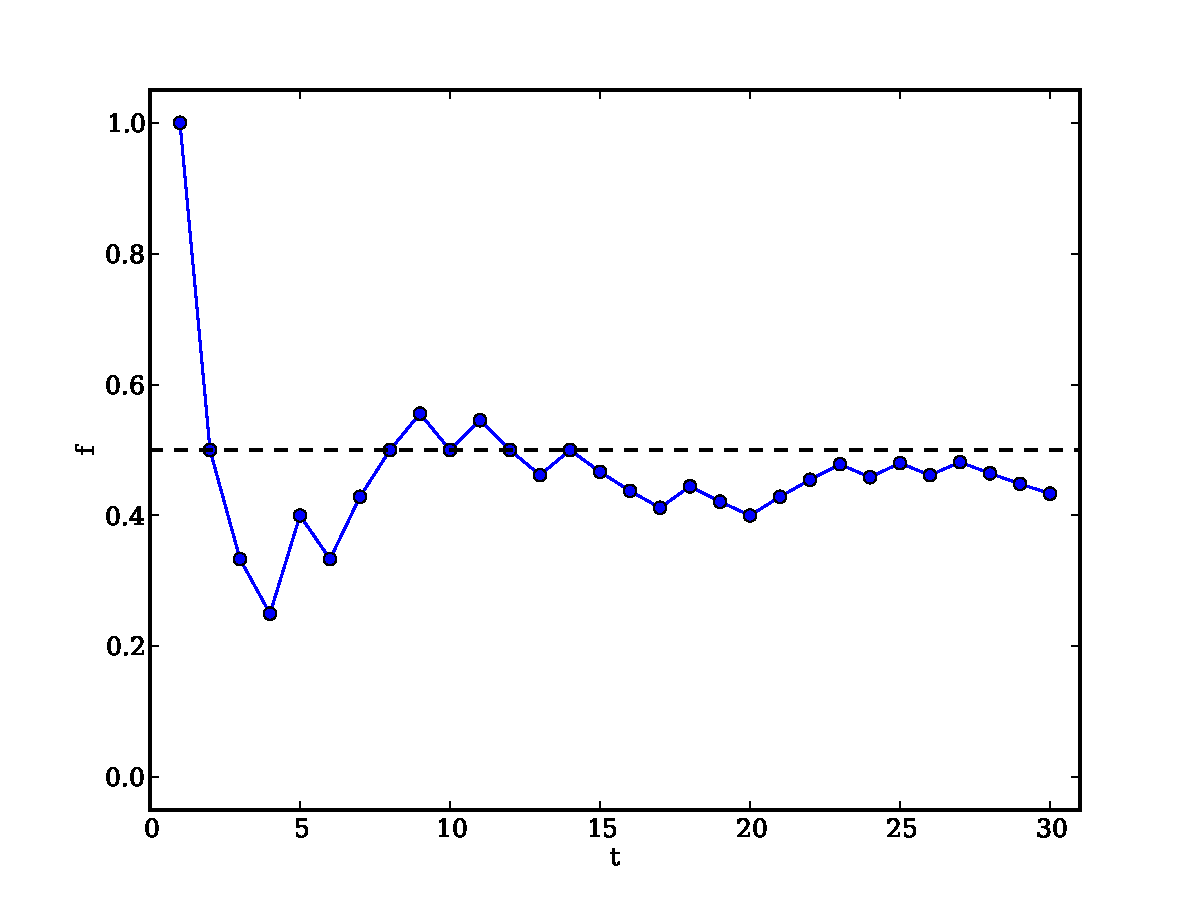
\includegraphics[width=0.75\textwidth]{Gr10-Probability-images/coin_toss_trials.pdf}
  \end{center}
%   \caption{Plot of the relative frequency of observing heads, $f$,
%     after having completed $t$ coin tosses.}
\end{figure}
\noindent
%english
% The graph above is the plot of the relative frequency of observing heads, $f$,
% after having completed $t$ coin tosses. It was generated from the table of numbers above
% by plotting the number of trials that have been completed, $t$, on the
% $x$-axis and the relative frequency, $f$, on the $y$-axis.

Die grafiek hierbo is die plot van die relatiewe frekwensie van die waarneming van om munte, $ f $ onder te hou,
na $ M $ muntstuk skiete. Dit was van die tafel hierbo gegenereer, deur die antaal toetse wat reeds voltooi is, $ T $, op die
$ x $-as te stip en die relatiewe frekwensie, $ f $, op die $ y $-as te stip.

Aan die begin (na 'n klein aantal toetse) fluktueer die relatiewe frekwensie baie rondom die teoretiese waarskynlikheid van $0,5$, aangetoon deur die gebroke lyn. Soos die aantal toetse toeneem fluktueer die relatiewe frekwensie al hoe minder en komal nader aan die teoretiese frekwensie.


}
\end{wex}

%\paragraph{eksperiment 2} Ons rol die twee dobbelstene $100$ kere en noteer telkens 
%die voorkoms van 'n som van $8$. Ons gebeurtenis kom $15$ kere voor. Hieruit kan ons die relatiewe frekwensie bereken as 
%\[\frac{15}{100}=0,15\]
%Hierdie is naby aan die teoretiese waarskynlikheid wat ons vroeer bereken het as $0,13\dot{8}$.

\begin{wex}{Relatiewe frekwensie en teoretiese waarskynlikheid}{
  Terwyl ons na $10$ sokker wedstryde kyk waar Span 1 teen Span 2 speel, teken ons die eindtellings aan:
    \begin{center}
      \begin{tabular}{lcccccccccc}
        \toprule
        Toets  & $1$ & $2$ & $3$ & $4$ & $5$ & $6$ & $7$ & $8$ & $9$ & $10$ \\
        \midrule
        Span 1 & $2$ & $0$ & $1$ & $1$ & $1$ & $1$ & $1$ & $0$ & $5$ & $3$ \\
        Span 2 & $0$ & $2$ & $2$ & $2$ & $2$ & $1$ & $1$ & $0$ & $0$ & $0$ \\
        \bottomrule
      \end{tabular}
    \end{center}
  Wat is die relatiewe frekwensie van Span 1 se wenne?
}{
  In hierdie eksperiment is elke toets in die vorm van 'n wedstryd tussen Span 1 en Span 2.

  \westep{Tel die aantal positiewe uitkomste}

  Ons stel belang in die gebeurtenis waar Span 1 wen. Uit die tabel sien ons dit gebeur $3$ keer.

  \westep{Bereken die relatiewe frekwensie}

  Daar is $10$ toetse in totaal. Dit beteken die relatiewe frekwensie van die gebeurtenis is \[\frac{3}{10} = 0,3\]
}
\end{wex}

Dit is belangrik om die verskil te verstaan tussen die teoretiese waarskynlikheid van 'n gebeurtenis en die gemete relatiewe frekwensie van die gebeurtenis in eksperimentele toetse. Die teoretiese waarskynlikheid is 'n getal wat ons kan bereken indien genoeg inligting oor die eksperiment beskikbaar is. Indien elke moontlike uitkoms in die monsterruimte ewekansig is, kan ons die aantal uitkomste in die gebeurtenis-versameling en die aantal uitkomste in die monsterruimte tel en daaruit die teoretiese waarskynlikheid bereken.\par

Die relatiewe frekwensie hang af van die volgorde van observasies gedurende 'n statistiese eksperiment. Die relatiewe frekwensie kan verskil telkens as die eksperiment herhaal word. Hoe meer toetse gedoen word gedurende 'n eksperiment, hoe nader kom die gemete relatiewe frekwensie aan die teoretiese frekwensie van die gebeurtenis.\par

So, waarom het ons statistiese ekpreimente nodig as daar reeds teoretiese waarskynlikhede bestaan? In sekere gevalle, soos ons sokker-eksperiment, is dit moeilik of onmoontlik om die teoretiese waarskynlikheid van 'n gebeurtenis te bereken. Aangesien ons nie met sekerheid weet of een span teen 'n ander gaan punte aanteken nie, is dit nie moontlik om die teoretiese waarskynlikheid van gebeurtenisse in sokker te bereken nie. In hierdie gevalle kan ons steeds die relatiewe frekwensie gebruik om die teoretiese waarskynlikheid te skat deur eksperimente te doen en die positiewe uitkomste te tel.

\section{Venn-diagramme}
'n Venn-diagram is a grafiese manier om verwantskappe tussen versamelings aan te dui. In elke Venn-diagram word 'n versameling aangedui deur 'n geslote kromme. Die area binne die kromme verteenwoordig die elemente van daardie versameling, terwyl die area buite die kromme die elemente bevat wat buite die versameling is.
\par


Venn-diagramme is handig om na te dink oor waarskynlikheid, aangesien ons met verskillende versamelings te doen het. Beskou twee gebeuretenisse, $A$ and $B$, in 'n monsterruimte $S$. Die figuur hieronder toon met behulp van Venn-diagramme die moontlike maniere waarop die gebeurtenis-versamelings kan oorvleuel:


\begin{figure}[H]
\begin{center}
\scalebox{1} % Change this value to rescale the drawing.
{
\begin{pspicture}(0,-1.701875)(10.96,1.721875)
\psframe[linewidth=0.04,dimen=outer](3.0,1.298125)(0.0,-1.701875)
\pscircle[linewidth=0.04,dimen=outer](0.78,-0.061875){0.56}
\pscircle[linewidth=0.04,dimen=outer](1.83,-0.371875){0.91}
\usefont{T1}{ptm}{m}{n}
\rput(0.7265625,0.728125){$A$}
\usefont{T1}{ptm}{m}{n}
\rput(1.8471875,0.768125){$B$}
\usefont{T1}{ptm}{m}{n}
\rput(2.8192186,1.528125){$S$}
\psframe[linewidth=0.04,dimen=outer](6.98,1.318125)(3.98,-1.681875)
\pscircle[linewidth=0.04,dimen=outer](4.7,-0.961875){0.56}
\pscircle[linewidth=0.04,dimen=outer](6.02,-0.001875){0.8}
\usefont{T1}{ptm}{m}{n}
\rput(4.7065625,-0.191875){$A$}
\usefont{T1}{ptm}{m}{n}
\rput(6.0071874,1.008125){$B$}
\usefont{T1}{ptm}{m}{n}
\rput(6.7992187,1.548125){$S$}
\psframe[linewidth=0.04,dimen=outer](10.96,1.318125)(7.96,-1.681875)
\pscircle[linewidth=0.04,dimen=outer](9.38,0.078125){0.56}
\pscircle[linewidth=0.04,dimen=outer](9.47,-0.271875){1.13}
\usefont{T1}{ptm}{m}{n}
\rput(10.266562,0.828125){$A$}
\usefont{T1}{ptm}{m}{n}
\rput(9.447187,-0.811875){$B$}
\usefont{T1}{ptm}{m}{n}
\rput(10.779219,1.548125){$S$}
\end{pspicture} 
}
%   \caption{Venn diagrams with different configurations of two events,
%     $A$ and $B$, in a sample space, $S$.}
\end{center}
\label{fig:venndiagrams}
\end{figure}\\

Die versamelings word aangedui deur 'n reghoek vir die monsterruimte $S$ en sirkels vir $A$ en $B$. In die eerste diagram oorvleuel die gebeurtenisse gedeeltelik. In die tweede diagram is daar geen oorvleueling nie. In die derde diagram bevat die een gebeurtenis die ander ten volle. Let op dat al die gebeurtenisse altyd binne die monsterruimte val, omdat die monsterruimte altyd al die moontlike uitkomste van die eksperiment bevat.\par
\mindsetvid{{V}enn diagrams and probabilities}{VMcbf}
\begin{wex}{Venn-diagramme}{
\wexlabel{wex:dice_venn}%
  Dui met behulp van 'n Venn-diagram die monsterruimte aan en die twee gebeurtenisse, $A$ en $B$, as twee dobbelstene gerol word:\\
\\
  Gebeurtenis $A:$ die som van die dobbelstene is gelyk aan $8$\\
 Gebeurtenis $B:$ ten minste een van die dobbelstene wys
    \raisebox{-2pt}{\begin{tikzpicture}
        \begin{scope}[scale=0.333]
          \makediegeneral{2}{}{0.175cm*0.333}
        \end{scope}
      \end{tikzpicture}}

}{
\begin{center}
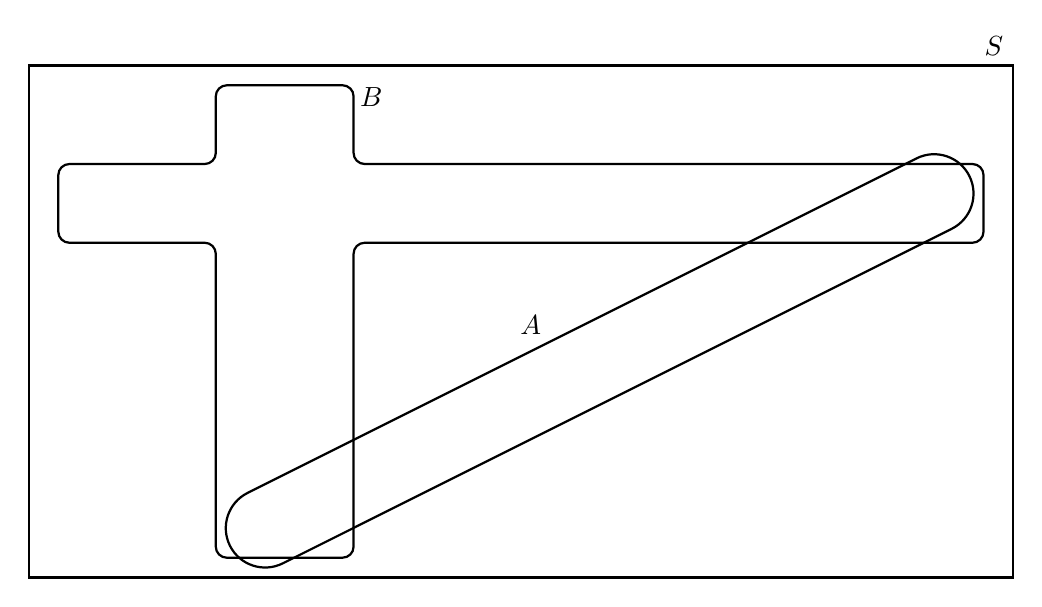
\begin{tikzpicture}
  \begin{scope}[scale=0.5]
    \begin{scope}[draw=gray,fill=gray]
      \foreach \x in {1, ..., 6} {
        \foreach \y in {1, ..., 6} {
          \pgfmathparse{15*rand} \let\rot\pgfmathresult
          \makediesmall{\x}{shift={(4cm*\x-0.66cm,-2cm*\y)},rotate=\rot}
          \pgfmathparse{15*rand} \let\rot\pgfmathresult
          \makediesmall{\y}{shift={(4cm*\x+0.66cm,-2cm*\y)},rotate=\rot}
        }
      }
    \end{scope}
    \draw[thick] (1.5cm, -0.5cm) rectangle (26.5cm, -13.5cm);
    \draw (26.5cm, -0.5cm) node[anchor=south east] {$S$};
    \draw[thick,rounded corners]
      (6.25cm, -1cm) -- (6.25cm, -3cm) -- (2.25cm, -3cm) -- (2.25cm, -5cm) --
      (6.25cm, -5cm) -- (6.25cm, -13cm) -- (9.75cm, -13cm) -- (9.75cm, -5cm) --
      (25.75cm, -5cm) -- (25.75cm, -3cm) -- (9.75cm, -3cm) -- (9.75cm, -1cm) -- cycle;
    \draw (10.2cm, -1.3cm) node {$B$};
    \begin{scope}[xshift=16cm,yshift=-8cm,rotate=26.57]
      \def\d{9.5cm}
      \def\r{1cm}
      \draw[thick]
        (+\d, +\r) -- (-\d, +\r) arc (90:270:\r) -- 
        (+\d, -\r) arc (-90:90:\r) -- cycle;
    \end{scope}
    \draw (14.25cm, -7.1cm) node {$A$};
  \end{scope}
\end{tikzpicture}
\end{center}
}
\end{wex}

%english wex below
\begin{wex}{Venn-diagramme}
{
\begin{minipage}{\textwidth}
Bepaal die stel van diamantkaarte wat uit 'n pak kaarte gehaal is. 'n Willekeurige kaart is uit die stel van diamante gekies.
\begin{itemize}
 \item Skyrf neer die monsterruimte, $S$, vir die eksperiment.
\item Wat is die waarde van $n(S)$?
\item Bepaal die volgende twee gebeurtenisse:
\begin{itemize}
\item $P$: 'n Ewige diamant is gekies
\item $R$: A prentkaart diamant is gekies
\end{itemize}
Stel monsterruimte $S$ en gebeurtenisse $P$ en $R$ met 'n Venn-diagram.
\end{itemize}
\end{minipage}
}
{
\westep{Skyrf neer die monsterruimte $S$}
\begin{align*}
S=\{A;~2;~3;~4;~5;~6;~7;~8;~9;~10;~J;~Q;~K\}
\end{align*}
\westep{Skryf neer die waarde van $n(S)$}
\begin{align*}
 n(S) = 13
\end{align*}
\westep{Teken die Venn-diagram}
\begin{center}
\scalebox{1} % Change this value to rescale the drawing.
{
\begin{pspicture}(0,-2.2)(4.5590625,2.2)
\pscircle[linewidth=0.04,dimen=outer](2.2,0.0){2.2}
\pscircle[linewidth=0.04,dimen=outer](1.45,-0.03){1.29}
\pscircle[linewidth=0.04,dimen=outer](2.54,0.76){0.9}
% \usefont{T1}{ptm}{m}{n}
\rput(3.7,1.9){$S$}
% \usefont{T1}{ptm}{m}{n}
\rput(2.9945312,0.83){$J$}
% \usefont{T1}{ptm}{m}{n}
\rput(2.4745312,1.29){$K$}
% \usefont{T1}{ptm}{m}{n}
\rput(2.1745312,0.53){$Q$}
% \usefont{T1}{ptm}{m}{n}
\rput(1.1445312,0.71){$2$}
% \usefont{T1}{ptm}{m}{n}
\rput(0.70453125,0.05){$4$}
% \usefont{T1}{ptm}{m}{n}
\rput(1.5645312,0.07){$6$}
% \usefont{T1}{ptm}{m}{n}
\rput(1.1245313,-0.55){$8$}
% \usefont{T1}{ptm}{m}{n}
\rput(2.0945313,-0.51){$10$}
% \usefont{T1}{ptm}{m}{n}
\rput(3.0845313,-0.77){$3$}
% \usefont{T1}{ptm}{m}{n}
\rput(3.8845313,-0.49){$5$}
% \usefont{T1}{ptm}{m}{n}
\rput(2.5445313,-1.45){$7$}
% \usefont{T1}{ptm}{m}{n}
\rput(3.4245312,-1.25){$9$}
% \usefont{T1}{ptm}{m}{n}
\rput(3.7745314,0.23){$A$}
% \usefont{T1}{ptm}{m}{n}
\rput(1.0145313,1.37){$P$}
% \usefont{T1}{ptm}{m}{n}
\rput(2.5045311,1.83){$R$}
\end{pspicture} 
}
\end{center}
}
\end{wex}
\begin{exercises}{}
{
  \begin{enumerate}[itemsep=5pt, label=\textbf{\arabic*}.]
  \item  Laat $S$ die versameling heelgetalle van $1$ tot $16$ aandui, $X$
    die versameling ewe getalle van $1$ tot $16$ en $Y$ die versameling priemgetalle van $1$ tot $16$
    \begin{enumerate}[noitemsep, label=\textbf{(\alph*)} ]
    \item Teken 'n Venn-diagram wat $S$, $X$ and $Y$ akkuraat aandui.
    \item Vind $n\left(S\right)$, $n\left(X\right)$, $n\left(Y\right)$,
      $n\left(X\cup Y\right)$, $n\left(X\cap Y\right)$.
    \end{enumerate}
  \item Daar is $79$ Graad $10$ leerders in die skool. Almal neem Wiskunde, Aardrykskunde of Geskiedenis. $41$ neem Aardrykskunde, $36$ neem Geskiedenis en $30$ neem Wiskunde. $16$ neem Wiskunde en Geskiedenis, $6$ neem Aardrykskunde en Geskiedenis, $8$ neem net Wiskunde en daar is $16$ wat slegs Geskiedenis neem.
    \begin{enumerate}[noitemsep, label=\textbf{(\alph*)} ]
    \item Teken 'n Venn-dagram om hierdie inligting te illustreer.
    \item Hoeveel leerders neem Wiskunde en Aardrykskunde, maar nie Geskiedenis nie?
    \item Hoeveel leerders neem net Aardrykskunde?
    \item Hoeveel leerders neem al drie vakke?
    \end{enumerate}
  \item Papiere word genommer van $1$ tot $12$ en in 'n houer geplaas en die houer geskud. Een papier op 'n slag word getrek en weer teruggeplaas.
    \begin{enumerate}[noitemsep, label=\textbf{(\alph*)} ]
    \item Wat is die monsterruimte, $S$?
    \item Skryf die versameling $A$ neer, wat die gebeurtenis voorstel van dietrek van 'n papier met 'n faktor van $12$.
    \item Skryf die versameling $B$ neer, wat die gebeuertenis voorstel van dietrek 'n papier, gemerk met 'n priemgetal.
    \item Gebruik 'n Venn-diagram om $A$, $B$ and $S$ voor te stel.
    \item Vind
      \begin{enumerate}[noitemsep, label=\textbf{\roman*.} ]
      \item $n\left(S\right)$
      \item $n\left(A\right)$
      \item $n\left(B\right)$

      \end{enumerate}

    \end{enumerate}
 \end{enumerate}

\insertpracticeinfo{3}
}
\end{exercises}

\section{Vereniging en interseksie}
\Definition{Vereniging}{Die vereniging van twee versamelings is 'n nuwe versameling wat al die elemente bevat wat minstens in een van die versamelings voorkom. Die vereniging word geskryf as $A \cup B$.}

\Definition{Deursit}{Die deursnit (of snyding of interseksie) van twee versamelings is 'n nuwe versameling wat al die elemente bevat wat in beide versamelings voorkom. Die interseksie word geskryf as $A \cap B$.}



Die figuur hieronder toon die vereniging en deursnit vir verskillende konfigurasies van twee gebeurtenisse in 'n monsterruimte met behulp van 'n Venn-diagram.

\begin{figure}[H]
  \begin{center}
  \begin{tabular}{ccc}
    \begin{tikzpicture}
      \begin{scope}[scale=3]
        \draw \samplespace; \labelsamplespace;
        \draw \circlepartiala; \labelpartiala;
        \draw \circlepartialb; \labelpartialb;
      \end{scope}
    \end{tikzpicture}
    &
    \begin{tikzpicture}
      \begin{scope}[scale=3]
        \draw \samplespace; \labelsamplespace;
        \draw \circleseparatea; \labelseparatea;
        \draw \circleseparateb; \labelseparateb;
      \end{scope}
    \end{tikzpicture}
    &
    \begin{tikzpicture}
      \begin{scope}[scale=3]
        \draw \samplespace; \labelsamplespace;
        \draw \circlefulla; \labelfulla;
        \draw \circlefullb; \labelfullb;
      \end{scope}
    \end{tikzpicture}
    \\
    \begin{tikzpicture}
      \begin{scope}[scale=3]
        \draw \samplespace; \labelsamplespace;
        \draw[fill=lightgray] (0.31369, 0.31041) arc (-162.62:130.73:0.3cm) arc (39.54:288.57:0.2cm);
        \draw[dotted] (0.31369, 0.31041) arc (197.38:130.73:0.3cm) arc (39.54:-71.43:0.2cm);
        \draw (0.4,0.7) node[anchor=south] {$A \cup B$};
      \end{scope}
    \end{tikzpicture}
    &
    \begin{tikzpicture}
      \begin{scope}[scale=3]
        \draw \samplespace; \labelsamplespace;
        \draw[fill=lightgray] \circleseparatea;
        \draw[fill=lightgray] \circleseparateb;
        \draw (0.3,0.2) node[anchor=west] {$A \cup B$};
      \end{scope}
    \end{tikzpicture}
    &
    \begin{tikzpicture}
      \begin{scope}[scale=3]
        \draw \samplespace; \labelsamplespace;
        \draw[fill=lightgray] \circlefulla;
        \draw[dotted] \circlefullb;
        \draw (0.5,0.83) node[anchor=south] {$A \cup B$};
      \end{scope}
    \end{tikzpicture}
    \\
    \begin{tikzpicture}
      \begin{scope}[scale=3]
        \draw \samplespace; \labelsamplespace;
        \draw[dotted] (0.31369, 0.31041) arc (-162.62:130.73:0.3cm) arc (39.54:288.57:0.2cm);
        \draw[fill=lightgray] (0.31369, 0.31041) arc (197.38:130.73:0.3cm) arc (39.54:-71.43:0.2cm);
        \draw (0.4,0.65) node[anchor=south] {$A \cap B$};
      \end{scope}
    \end{tikzpicture}
    &
    \begin{tikzpicture}
      \begin{scope}[scale=3]
        \draw \samplespace; \labelsamplespace;
        \draw[dotted] \circleseparatea;
        \draw[dotted] \circleseparateb;
      \end{scope}
    \end{tikzpicture}
    &
    \begin{tikzpicture}
      \begin{scope}[scale=3]
        \draw \samplespace; \labelsamplespace;
        \draw[dotted] \circlefulla;
        \draw[fill=lightgray] \circlefullb;
        \draw (0.5,0.75) node[anchor=south] {$A \cap B$};
      \end{scope}
    \end{tikzpicture}
    \\
  \end{tabular}
\end{center}

  \begin{caption*}{Die verenigings en interseksies van verskillende gebeurtenisse. Let op dat die middelste kolom, die interseksie van $A \cap B$, leeg is aangesien die twee versamelings nie oorvleuel nie. Verder, in die laaste kolom is die vereniging, $A \cup B$, gelyk aan $A$ en die interseksie, $A \cap B$, gelyk aan $B$ aangesien $B$ ten volle bevat word deur $A$.}\end{caption*}
  \label{fig:venn_union_intersection}
\end{figure}
\par

\mindsetvid{Inclusive and exclusive events}{VMcci}


\section{Waarskynlikheids-identiteite}

  \[P(S)=1\]


Die monsterruimte bevat per definisie alle moontlike uitkomste van 'n eksperiment. Ons weet dus dat die waarskynlikheid van 'n resultaat uit 'n monsterruimte $1$ is.


  \[P(A \cup B) = P(A) + P(B) - P(A \cap B)\]


Ons sal hierdie identiteit bewys deur die Venn-diagramme hierbo te gebruik. Vir elk van die $4$ terme in die verenigings-identiteit kan ons 'n Venn-diagram teken en telkens die verskillende diagramme bytel of aftrek. Die area van 'n gebied verteenwoordig sy waarskynlikheid.\par

Ons doen hierdie vir die eerste diagram van die Venn-diagram hierbo. Jy kan dit self probeer vir die ander kolomme.

\begin{center}
\begin{tabular}{m{0.5cm}m{1.5cm}m{0.5cm}m{0.3cm}@{\hspace{0.1cm}}m{1.5cm}m{0.5cm}m{1.5cm}@{\hspace{0.1cm}}m{0.3cm}}
   & $P(A)$ & $+$ && $P(B)$ & $-$ & $P(A \cap B)$ \\[4pt]
 = & \begin{tikzpicture}
   \begin{scope}[scale=1.5]
     \draw \samplespace;
     \draw[fill=lightgray] \circlepartiala;
   \end{scope}
\end{tikzpicture} & $+$ & $\Bigg($ & \begin{tikzpicture}
   \begin{scope}[scale=1.5]
     \draw \samplespace;
     \draw[fill=lightgray] \circlepartialb;
   \end{scope}
\end{tikzpicture} & $-$ & \begin{tikzpicture}
   \begin{scope}[scale=1.5]
     \draw \samplespace;
     \draw[fill=lightgray] (0.31369, 0.31041) arc (197.38:130.73:0.3cm) arc (39.54:-71.43:0.2cm);
   \end{scope}
\end{tikzpicture} & $\Bigg)$ \\[4pt]
 = & \begin{tikzpicture}
   \begin{scope}[scale=1.5]
     \draw \samplespace;
     \draw[fill=lightgray] \circlepartiala;
   \end{scope}
\end{tikzpicture} & $+$ && \begin{tikzpicture}
   \begin{scope}[scale=1.5]
     \draw \samplespace;
     \draw[fill=lightgray] (0.31369, 0.31041) arc (-162.62:130.73:0.3cm) arc (39.54:-71.43:0.2cm);
   \end{scope}
\end{tikzpicture} \\[4pt]
 = & \begin{tikzpicture}
      \begin{scope}[scale=1.5]
        \draw \samplespace;
        \draw[fill=lightgray] (0.31369, 0.31041) arc (-162.62:130.73:0.3cm) arc (39.54:288.57:0.2cm);
      \end{scope}
\end{tikzpicture} \\[4pt]
 = & $P(A \cup B)$
\end{tabular}
\end{center}

\begin{wex}{Vereniging en deursnit van gebeurtenisse}{
  Vergelyk die waarskynlikhede van gebeurtenisse $A$ and $B$ in die Voorbeeld \wexref{wex:dice_venn} en toon aan dat die identiteit 
\[P(A \cup B) = P(A) + P(B) - P(A \cap B)\]
bevredig word.

}{
  \westep{Skryf die waarskynlikhede van die twee gebeurtenisse, hulle vereniging en hulle deursnit.}
  
Uit die figuur in Voorbeeld \wexref{wex:dice_venn} kan ons die aantal uitkomste in elke gebeurtenis tel. Om die waarskynlikheid van 'n gebeurtenis te verkry deel ons die grootte van die gebeurtenis deur die grootte van sy monsterruimte wat $n(S)=36$ is.
  \[\begin{array}{r@{$\ =\ $}c@{$\ =\ $}l}
    P(A)        & \dfrac{n(A)}{n(S)}        & \dfrac{5}{36}  \\[8pt]
    P(B)        & \dfrac{n(B)}{n(S)}        & \dfrac{11}{36} \\[8pt]
    P(A \cap B) & \dfrac{n(A \cap B)}{n(S)} & \dfrac{2}{36}  \\[8pt]
    P(A \cup B) & \dfrac{n(A \cup B)}{n(S)} & \dfrac{14}{36}
  \end{array}\]
  % Sorry for the ugly equation: didn't know how to make the alignment
  % work otherwise

% gmf

  \westep{Skryf die identiteit neer kontroleer dit.}
  \begin{eqnarray*}
    P(A \cup B) &=& P(A) + P(B) - P(A \cap B) \\
    \frac{14}{36} &=& \frac{5}{36} + \frac{11}{36} - \frac{2}{36} \\
    &=& \frac{5}{36} + \frac{9}{36} \\
    &=& \frac{14}{36} \qquad\qquad
  \end{eqnarray*}
}
\end{wex}

\section{Onderlinge uitsluitende gebeurtenisse}
\Definition{Onderlinge uitsluitende gebeurtenisse}{Twee gebeurtenisse is onderling uitlsluitende indien hulle nie saam kan voorkom nie. Wanneer die uitkoms van 'n eksperiment in eerste gebeurtenis val, kan dit nie ook in die tweede gebeurtenis wees nie.}

'n Ander manier om dit te beskrywe is om te s\^e dat die twee gebeurtenis-versamelings, $A$ en $B$, nie elemente in gemeen kan h\^e nie, of $P(A \cap B) = \emptyset$
(waar $\emptyset$ die lee versameling aandui).

Ons het alreeds die Venn-diagramme van onderlinge uitsluitende gebeurtenisse gesien in die middelkolom van die Venn diagramme op bladsy \pageref{fig:venn_union_intersection}.

\begin{figure}[H]
  \begin{center}
  \begin{tabular}{ccc}
    \begin{tikzpicture}
      \begin{scope}[scale=3]
        \draw \samplespace; \labelsamplespace;
        \draw \circleseparatea; \labelseparatea;
        \draw \circleseparateb; \labelseparateb;
      \end{scope}
    \end{tikzpicture}
    &
    \begin{tikzpicture}
      \begin{scope}[scale=3]
        \draw \samplespace; \labelsamplespace;
        \draw[fill=lightgray] \circleseparatea;
        \draw[fill=lightgray] \circleseparateb;
        \draw (0.3,0.2) node[anchor=west] {$A \cup B$};
      \end{scope}
    \end{tikzpicture}
    &
    \begin{tikzpicture}
      \begin{scope}[scale=3]
        \draw \samplespace; \labelsamplespace;
        \draw[dotted] \circleseparatea;
        \draw[dotted] \circleseparateb;
        \draw (1,1) node[anchor=south east] {$A \cap B$};
      \end{scope}
    \end{tikzpicture}
  \end{tabular}
\end{center}

%   \caption{Onderlinge uitsluitlike gebeurtenisse.}
\end{figure}

Uit hierdie figuur kan mens sien dat die interseksie geen elemente het nie. Mens kan ook sien dat die waarskynlikheid van die vereniging die som is van van die waarskynlikhede van die gebeurtenisse.
\[P(A \cup B) = P(A) + P(B)\]
Hierdie verwantskap geld slegs vir onderlinge uitsluitende gebeurtenisse.

\begin{wex}{Onderling uitsluitende gebeurtenisse}{
\begin{minipage}{\textwidth}
  Ons rol twee dobbelstene en stel belang in die volgende twee gebeurtenisse:
  \begin{itemize}
  \item[] $A:$ Die getalle op die twee dobbelstene se som is $8$
  \item[] $B:$ Ten minste een dobbesteen wys 
    \raisebox{-2pt}{\begin{tikzpicture}
        \begin{scope}[scale=0.333]
          \makediegeneral{1}{}{0.175cm*0.333}
        \end{scope}
      \end{tikzpicture}}
  \end{itemize}
  Toon aan dat die gebeurtenisse onderling uitsluitend is.
\end{minipage}
}{
  \westep{Teken die monsterruimte en die twee gebeurtenisse}

\begin{center}
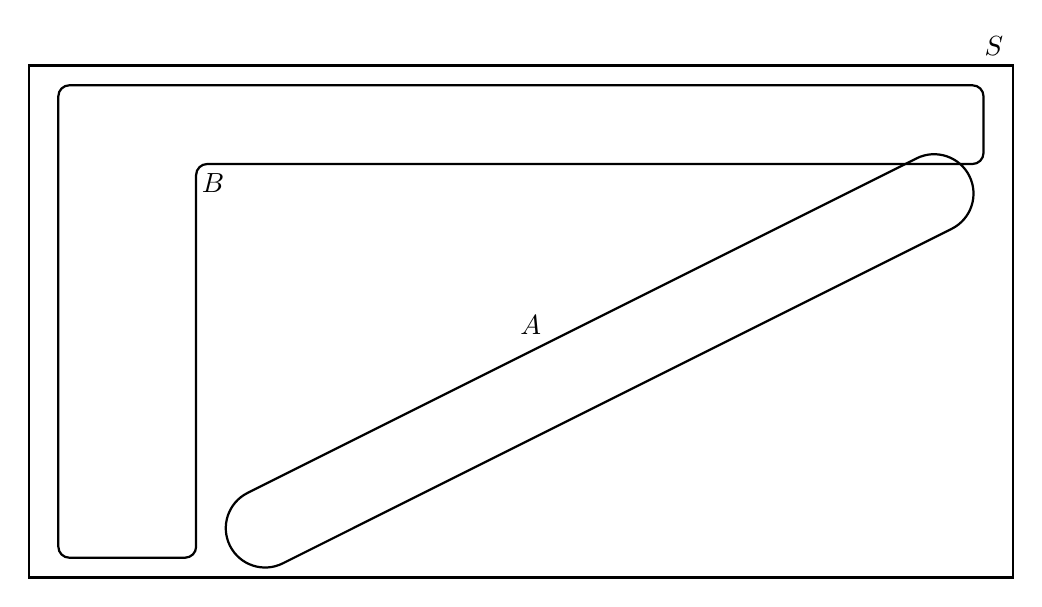
\begin{tikzpicture}
  \begin{scope}[scale=0.5]
    \begin{scope}[draw=gray,fill=gray]
      \foreach \x in {1, ..., 6} {
        \foreach \y in {1, ..., 6} {
          \pgfmathparse{15*rand} \let\rot\pgfmathresult
          \makediesmall{\x}{shift={(4cm*\x-0.66cm,-2cm*\y)},rotate=\rot}
          \pgfmathparse{15*rand} \let\rot\pgfmathresult
          \makediesmall{\y}{shift={(4cm*\x+0.66cm,-2cm*\y)},rotate=\rot}
        }
      }
    \end{scope}
    \draw[thick] (1.5cm, -0.5cm) rectangle (26.5cm, -13.5cm);
    \draw (26.5cm, -0.5cm) node[anchor=south east] {$S$};
    \draw[thick,rounded corners]
      (2.25cm, -1cm) -- (2.25cm, -13cm) -- (5.75cm, -13cm) -- (5.75cm, -3cm) --
      (25.75cm, -3cm) -- (25.75cm, -1cm) -- cycle;
    \draw (5.65cm, -3cm) node[anchor=north west] {$B$};
    \begin{scope}[xshift=16cm,yshift=-8cm,rotate=26.57]
      \def\d{9.5cm}
      \def\r{1cm}
      \draw[thick]
        (+\d, +\r) -- (-\d, +\r) arc (90:270:\r) -- 
        (+\d, -\r) arc (-90:90:\r) -- cycle;
    \end{scope}
    \draw (14.25cm, -7.1cm) node {$A$};
  \end{scope}
\end{tikzpicture}
\end{center}

  \westep{Bepaal die interseksie}

Uit die figuur sien ons dat daar geen elemente in gemeen in $A$ and $B$ is nie. Die gebeurtenisse is dus onderling uitsluitende.
}
\end{wex}

\section{Komplement\^ere gebeurtenisse}

\Definition{Komplement\^ere versameling}{Die komplement van 'n versameling, $A$, is 'n ander versameling wat al die elemente bevat wat nie in 
  $A$ is nie. Ons skryf die komplement van $A$ as $A'$, of soms ``$\mbox{nie}(A)$''.}

Vir 'n eksperiment met 'n monsterruimte $S$ en 'n gebeurtenis $A$, kan ons sekere identiteite aflei vir komplement\^ere gebeurtenisse. Aangesien elke element van $A$ nie in $A'$ voorkom nie, weet ons dat komplementere gebeurtenisse onderling uitsluitende is.


  \[A \cap A' = \emptyset\]


Aangesien elke element van die monsterruimte of in $A$ of in $A'$ voorkom, omvat die vereniging van komplementere gebeurtenisse die monsterruimte.

  \[A \cup A' = S\]


Uit die vorige twee identiteite weet ons dat die waarskynlikhede van komplement\^ere gebeurtenisse saam gelyk is aan $1$.


  \[P(A) + P(A') = P(A \cup A') = P(S) = 1\]


\mindsetvid{Complementary events}{VMcdl}

\begin{wex}{Beredenering met belhulp van Venn-diagramme}{
\begin{minipage}{\textwidth}
  In 'n opname is $70$ mense gevra watter produk hulle gebruik: A of B of beide. Die verslag toon dat $25$ mense produk A gebruik, $35$ mense produk B gebruik en $15$ mense gebruik nie een nie. Gebruik 'n Venn-diagram om te bereken hoeveel mense:
  \begin{enumerate}[itemsep=3pt, label=\textbf{\arabic*}.]
\item gebruik slegs produk $A$
  \item gebruik slegs produk B
  \item gebruik beide produk A en produk B
  \end{enumerate}
\end{minipage}
}{
\begin{minipage}{\textwidth}
  \westep{Bepaal die groottes van die monsterruimte, die gebeurtenis-versamelings, hule vereniging en hulle deursnit}
  \begin{itemize}
  \item Ons weet $70$ mense het deelgeneem, dus is die grootte van die monsterruimte $n(S) = 70$.
  \item Ons weet $25$ mense gebruik produk A, dus is $n(A) = 25$.
  \item Ons weet $35$ mense gebruik produk B, dus is $n(B) = 35$.
  \item Ons weet $15$ mense gebruik nie een van die produkte nie. Dit beteken dat minstens $70-15=55$ mense ten minste een van die produkte gebruik, dus is 
    $n(A \cup B) = 55$.
  \item Ons weet nie hoeveel mense beide produkte gebruik nie, dus moet ons die grootte van die deursnit $A \cap B$ bereken, deur die volgende identiteit te gebruik
    \begin{eqnarray*}
      P(A \cup B) & = & P(A) + P(B) - P(A \cap B) \\
      \frac{n(A \cup B)}{n(S)} & = & \frac{n(A)}{n(S)} + \frac{n(B)}{n(S)} - \frac{n(A \cap B)}{n(S)} \\
      \frac{55}{70} & = & \frac{25}{70} + \frac{35}{70} - \frac{n(A \cap B)}{70} \\
      \therefore n(A \cap B) & = & 25 + 35 - 55 \\
      & = & 5
    \end{eqnarray*}
  \end{itemize}


  \westep{Bepaal of die gebeurtenisse onderling uitsluitend is}
Aangesien die interseksie, $A \cap B$, nie leeg is nie, is die gebeurtenisse nie onderling uisluitend nie. Dit beteken dat hulle sirkels behoort te oorvleuel in die Venn-diagram.

  \westep{Teken die Venn-diagram en vul die getalle in}
    \begin{center}
      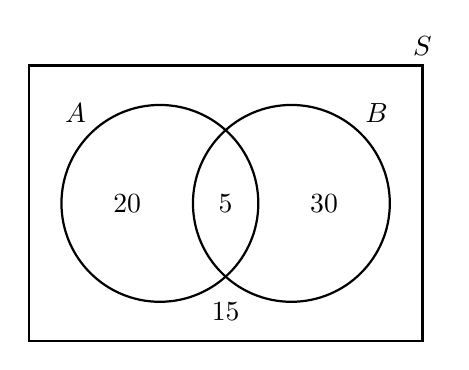
\begin{tikzpicture}
        \begin{scope}[scale=5]
          \draw[thick] (0, 0) rectangle (1cm, 0.7cm);
          \draw (1cm, 0.7cm) node[anchor=south] {$S$};
          \draw[thick] (0.333cm, 0.35cm) circle (0.25cm);
          \draw (0.17, 0.53) node[anchor=south east] {$A$};
          \draw[thick] (0.667cm, 0.35cm) circle (0.25cm);
          \draw (0.83, 0.53) node[anchor=south west] {$B$};
          % Numbers
          \draw (0.5, 0.35) node {$5$};
          \draw (0.25, 0.35) node {$20$};
          \draw (0.75, 0.35) node {$30$};
          \draw (0.5, 0.075) node {$15$};
        \end{scope}
      \end{tikzpicture}
    \end{center}

  \westep{Lees die antwoorde}
  \begin{enumerate}[itemsep=5pt, label=\textbf{\arabic*}.]
  \item $20$ mense gebruik slegs produk A.
  \item $30$ mense gebruik slegs produk B.
  \item $5$ mense gebruik beide produkte.
  \end{enumerate}
\end{minipage}
}
\end{wex}

\begin{exercises}{}
{
  \begin{enumerate}[itemsep=3pt, label=\textbf{\arabic*}.]
  \item  'n Kas bevat gekleurde blokkies. Die aantal van elke kleur word in die onderstaande tabel aangedui.

  \begin{center}
      \begin{tabular}{|l|c|c|c|c|}
        \hline
        \textbf{Kleur} & Pers & Oranje & Wit & Pink \\ \hline
       
        \textbf{Aantal blokkies} & $24$ & $32$ & $41$ & $19$ \\ \hline
   
      \end{tabular}
    \end{center}
    'n Blokkie word willekeurig gekies. Wat is die waarskynlikheid dat die blokkie die volgende kleur sal wees:
    \begin{enumerate}[noitemsep, label=\textbf{(\alph*)} ]
    \item pers
    \item pers of wit
    \item pienk en oranje
    \item nie oranje?
    \end{enumerate}

  \item 'n Klein skooltjie het 'n klas met kinders van verskillende ouderdomme. Die tabel gee die aantal kinders van elke ouderdom in die klas.

    \begin{center}
      \begin{tabular}{|l|c|c|c|}
        \hline
               & $3$ jaar oud & $4$ jaar oud & $5$ jaar oud \\\hline
   
        \textbf{manlik}   & $2$ & $7$ & $6$ \\\hline
        \textbf{vroulik} & $6$ & $5$ & $4$ \\\hline
       
      \end{tabular}
    \end{center}

    As 'n leerder lukraak gekies word, wat is die waarskynlikheid dat die leerder die volgende sal wees:
    \begin{enumerate}[noitemsep, label=\textbf{(\alph*)} ]
    \item vroulik
    \item 'n $4$ jaar oud en manlik 
    \item $3$ of $4$ jaar oud
    \item $3$ en $4$ jaar oud
    \item nie $5$
    \item $3$ of vroulik?
    \end{enumerate}

  \item Fiona het $85$ skyfies, genommer van $1$ to
    $85$. Indien 'n skyfie willekeurig gekies word, wat is die waarskynlikheid dat die nommer: 
    \begin{enumerate}[noitemsep, label=\textbf{(\alph*)} ]
    \item eindig met $5$
    \item vermenigvuldig kan word met $3$
    \item vermenigvuldig kan word met  $6$
    \item $65$ is
    \item nie 'n veelvoud van $5$ is nie
    \item 'n veelvoud van $4$ of $3$ is
    \item 'n veelvoud van $2$ en $6$ is
    \item  $1$ is?
    \end{enumerate}
  \end{enumerate}

\insertpracticeinfo{3}
}
\end{exercises}

%summary all in english!
\summary{VMdve}
\begin{itemize}
\item ’n Eksperiment verwys na ’n proses met onsekerheid.

\item Die uitslag van ’n eksperiment is ’n enkele resultaat van daardie eksperiment.


\item Die monsterruimte van ’n versameling is die versameling van al die moontlike uitslae
van daardie eksperiment. Die monsterruimte word aangedui deur die simbool $S$ en
die grootte van die monsterruimte (die som van al die moontlike uitkomste) word
aangedui deur

  $n(S)$.

\item ’n Gebeurtenis is ’n spesifieke versameling van uitkomste van ’n eksperiment waarin
jy belangstel. ’n Gebeurtenis word aangedui deur die letter $E$ en die aantal uitkomste
van die gebeurtenis met
 $n(E)$.

\item ’n Waarskynlikheid is ’n reële getal tussen $0$ en $1$ wat beskryf hoe waarskynlik dit is
dat die gebeurtenis sal plaasvind.

\begin{itemize}
\item ’n Waarskynlikheid van $0$ beteken dat die gebeurtenis nooit sal plaasvind nie.

\item ’n Waarskynlikheid van $1$ beteken dat die gebeurtenis altyd sal plaasvind.

\item ’n Waarskynlikheid van $0,5$ beteken dat die gebeurtenis die helfte van die tyd sal plaasvind, of
$1$ keer uit elke $2$.

\end{itemize}

\item Die relatiewe frekwensie van ’n gebeurtenis word gedefinieer as die aantal kere wat
die gebeurtenis voorkom in ’n aantal eksperimente, gedeel deur die aantal eksperi-
mente.


\item Die vereniging van twee versamelings is ’n nuwe versameling wat al die elemente
bevat wat minstens in een van die versamelings voorkom. Die vereniging word
geskryf as
 $A \cup B$.

\item Die deursnit (of snyding of interseksie) van twee versamelings is ’n nuwe versameling
wat al die elemente bevat wat in beide versamelings voorkom. Die interseksie word
geskryf as
 $A \cap B$.

\item Die waarskynlikheid van monsterruimte:  $P(S)=1$.

\item Vereniging en deursnit: $P(A \cup B) = P(A) + P(B) - P(A \cap B)$.


\item Twee gebeurtenisse is onderling uitlsluitende indien hulle nie saam kan voorkom
nie. Wanneer die uitkoms van ’n eksperiment in eerste gebeurtenis val, kan dit nie
ook in die tweede gebeurtenis wees nie.



\item Die komplement van ’n versameling, $A$, is ’n ander versameling wat al die elemente
bevat wat nie in $A$ is nie. Ons skryf die komplement van $A$ as $A'$ , of soms “nie($A$)”.


\item Komplementêre gebeurtenisse is onderling uitsluitende: $A \cap A' = \emptyset$.


\item Komplementêre gebeurtenisse bedek dieselfde monsterruimte:
$A \cup A' = S$.


\item Die waarskynlikhede van komplementêre gebeurtenisse
saam gelyk is
 $1$: $P(A) + P(A') = P(A \cup A') = P(S) = 1$.

\end{itemize}
\begin{eocexercises}{Waarskynlikheid}
  \begin{enumerate}[itemsep=5pt, label=\textbf{\arabic*}.]
  \item 'n Groep van $45$ kinders is gevra of hulle  Frosties en/of
    Strawberry Pops eet. $31$ eet beide en $6$ eet net Frosties.  Wat is die waarskynlikheid dat 'n kind wat lukraak gekies word net Strawberry
    Pops eet?
  \item In 'n groep van $42$ leerders het almal behalwe $3$ 'n pakkie skyfies of 'n Fanta of beide gehad. As $23$ 'n pakkie skyfies gehad het, en $7$ hiervan het ook 'n Fanta gehad, wat is die waarskynlikheid dat 'n leerder wat willekeurig gekies word die volgende het:
    \begin{enumerate}[noitemsep, label=\textbf{(\alph*)} ]
    \item beide skyfies en Fanta
    \item net Fanta
    \end{enumerate}
  \item Gebruik 'n Venn-diagram om die volgende waarskynlikhede van 'n dobbelsteen wat gerol word te bereken:
    \begin{enumerate}[noitemsep, label=\textbf{(\alph*)} ]
    \item 'n veelvoud van $5$ en 'n onewe getal
    \item 'n getal wat nie 'n veelvoud van $5$ is nie en ook nie 'n onewe getal nie
    \item 'n getal wat nie 'n veelvoud van $5$ is nie, maar onewe.
    \end{enumerate}
  \item 'n Pakkie het geel en pienk lekkers. Die waarskynlikheid om 'n pienk lekker te kies is $\frac{7}{12}$.
Wat is die waarskynlikheid om 'n geel lekker uit te haal?

  \item In 'n parkeerterrein met $300$ motors is daar $190$ Opels. Wat is die waarskynlikheid dat die eerste motor wat uitry die volgende is:
    \begin{enumerate}[noitemsep, label=\textbf{(\alph*)} ]
    \item 'n Opel
    \item nie 'n Opel
    \end{enumerate}
  \item Tamara het $18$ los sokkies in 'n laai. Agt van hierdie is oranje en twee pienk. Bereken die waarskynlikheid dat die eerste sokkie wat willekeurig gekies word die volgende is:
    \begin{enumerate}[noitemsep, label=\textbf{(\alph*)} ]
    \item Oranje
    \item nie oranje
    \item pienk
    \item nie pienk
    \item oranje of pienk
    \item nie oranje of pienk
    \end{enumerate}
  \item Daar is $9$ brosbrood koekies, $4$ gemmerkoekies,
    $11$ sjokoladekoekies en $18$ Jambos op 'n bord. As 'n koekie willekeurig gekies word, wat is die waaarskynlikheid dat:
    \begin{enumerate}[noitemsep, label=\textbf{(\alph*)} ]
    \item dit 'n gemmerkoekie of 'n Jambo is?
    \item dit nie 'n brosbroodkoekie is nie?
    \end{enumerate}
  \item $280$ kaartjies is verkoop in 'n lotery. Ingrid het $15$ gekoop. Wat is die waarskynlikheid dat Ingrid:
    \begin{enumerate}[noitemsep, label=\textbf{(\alph*)} ]
    \item die prys wen
    \item nie die prys wen nie
    \end{enumerate}
  \item Die kinders in 'n kleuterskool is geklassifiseer per haarkleur en oogkleur. $44$ het rooi hare en nie bruin oe nie, $14$ het bruin oe maar nie rooi hare nie en $40$ het nie bruin oe of rooi hare nie.
    \begin{enumerate}[noitemsep, label=\textbf{(\alph*)} ]
    \item Hoeveel kinders is in die skool?
    \item Wat is die waarskynlikheid dat 'n kind wat willekeurig gekies word die volgende het:
      \begin{enumerate}[noitemsep, label=\roman*. ]
      \item bruin o\"e
      \item rooi hare
      \end{enumerate} 
    \item 'n Kind met bruin\"e word willekeurig gekies. Wat is die waarskynlikheid dat hierdie kind rooi hare het?
    \end{enumerate}
  \item 'n Houer bevat pers, blou en swart lekkers. Die waarskynlikheid dat 'n lekker wat willekeurig gekies word pers is, is $\frac{1}{7}$, en die waarskynlikheid dat dit swart sal wees is $\frac{3}{5}$.
    \begin{enumerate}[noitemsep, label=\textbf{(\alph*)} ]
    \item As ek 'n lekker willekeurig kies, wat is die waarskynlikheid dit die volgende sal wees:
      \begin{enumerate}[noitemsep, label=\roman*. ]
      \item pers of blou
      \item swart
      \item pers
      \end{enumerate}
    \item As daar $70$ lekkers in die houer is, hoeveel perses is daar?
    \item $\frac{2}{5}$ van die pers lekkers in (b) het strepe en die res nie, hoeveel pers lekkers het strepe?
    \end{enumerate}
  \item Vir elk van die volgende, teken 'n Venn-diagram om die situasie voor te stel en vind 'n voorbeeld ter illustrasie.
    \begin{enumerate}[noitemsep, label=\textbf{(\alph*)} ]
    \item 'n monsterruimte waarin daar twee gebeurtenisse is wat nie ondeling uitsluitend is nie.
    \item 'n monsterruimte waarin daar twee komplementere gebeurtenisse is.
    \end{enumerate}
  \item Gebruik 'n Venn-diagram om te bewys dat die waarskynlikheid van voorkoms van gebeurtenis  $A$ of $B$ ($A$ en $B$ is nie onderling uitsluitend nie) gegee word deur:
    \[P(A \cup B) = P(A) + P(B) - P(A \cap B)\]
  \item Al die klawerkaarte word uit 'n pak kaarte gehaal. Die res word dan geskommel en een kaart gekies. Die kaart word dan teruggeplaas voor die volgende een gekies word.
    \begin{enumerate}[noitemsep, label=\textbf{(\alph*)} ]
    \item Wat is die monsterruimte?
    \item Vind 'n versameling om gebeurtenis $P$, die trek van 'n prentkaart, voor te stel.
    \item Vind 'n versameling om gebeurtenis $N$, die trek van 'n nommerkaart, voor te stel.
    \item Vertoon die bostaande gebeurtenisse in 'n Venn-diagram.
    \item Wat is 'n goeie beskrywing van die versamelings $P$ en $N$?
      (Wenk: Vind enige elemente van $P$ in $N$ en van $N$ in $P$.)
    \end{enumerate}

%english questions below
  \item 'n Opname was by Mutende Primêre Skool uitgevoer om vas te stel hoeveel van die $ 650 $ leerders vetkoek, en hoeveel lekkers tydens pouse koop. Die volgende was bevind:
% A survey was conducted at Mutende Secondary school to establish how many of the $650$ learners buy vetkoek and how many buy sweets during break. The following was found:
\begin{itemize}
 \item $50$ leerders het niks gekoop nie
\item $400$ leerders het vetkoek gekoop
\item $300$ leerders het lekkers gekoop
\end{itemize}
\begin{enumerate}[noitemsep, label=\textbf{(\alph*)} ]
 \item Vertoon hierdie inligting met 'n Venn-diagram
\item Indien 'n leerder willekeurig gekies is, bereken die waarskynlikheid dat die leerder koop:
% If a learner is chose randomly, calculate the probability that this learner buys:
\begin{enumerate}[noitemsep, label=\roman*. ]
 \item net lekkers
\item net vetkoek
\item nie vetkoek en nie lekkers nie
\item vetkoek en lekkers
\item vetkoek of lekkers
\end{enumerate}
\end{enumerate}
\item In 'n opname by Lwandani se Sekondêre Skool is $80$ mense gevra of hulle die Sowetan of die Daily Sun of albei koerante lees. Die verslag toondat $45$ mense die Daily Sun lees, $30$ die Sowetan lees en $10$ lees nie een van hulle nie. Gebruik 'n Venn-diagram om die persentasie van mense te vind wat:
\begin{enumerate}[noitemsep, label=\textbf{(\alph*)} ]
 \item net die Daily Sun lees
\item net die Sowetan lees
\item die Daily Sun en die Sowetan lees
\end{enumerate}

  \end{enumerate}

\insertpracticeinfo{15}
\end{eocexercises}
